% Options for packages loaded elsewhere
\PassOptionsToPackage{unicode}{hyperref}
\PassOptionsToPackage{hyphens}{url}
%
\documentclass[
  ignorenonframetext,
]{beamer}
\usepackage{pgfpages}
\setbeamertemplate{caption}[numbered]
\setbeamertemplate{caption label separator}{: }
\setbeamercolor{caption name}{fg=normal text.fg}
\beamertemplatenavigationsymbolsempty
% Prevent slide breaks in the middle of a paragraph
\widowpenalties 1 10000
\raggedbottom
\setbeamertemplate{part page}{
  \centering
  \begin{beamercolorbox}[sep=16pt,center]{part title}
    \usebeamerfont{part title}\insertpart\par
  \end{beamercolorbox}
}
\setbeamertemplate{section page}{
  \centering
  \begin{beamercolorbox}[sep=12pt,center]{part title}
    \usebeamerfont{section title}\insertsection\par
  \end{beamercolorbox}
}
\setbeamertemplate{subsection page}{
  \centering
  \begin{beamercolorbox}[sep=8pt,center]{part title}
    \usebeamerfont{subsection title}\insertsubsection\par
  \end{beamercolorbox}
}
\AtBeginPart{
  \frame{\partpage}
}
\AtBeginSection{
  \ifbibliography
  \else
    \frame{\sectionpage}
  \fi
}
\AtBeginSubsection{
  \frame{\subsectionpage}
}
\usepackage{lmodern}
\usepackage{amssymb,amsmath}
\usepackage{ifxetex,ifluatex}
\ifnum 0\ifxetex 1\fi\ifluatex 1\fi=0 % if pdftex
  \usepackage[T1]{fontenc}
  \usepackage[utf8]{inputenc}
  \usepackage{textcomp} % provide euro and other symbols
\else % if luatex or xetex
  \usepackage{unicode-math}
  \defaultfontfeatures{Scale=MatchLowercase}
  \defaultfontfeatures[\rmfamily]{Ligatures=TeX,Scale=1}
\fi
% Use upquote if available, for straight quotes in verbatim environments
\IfFileExists{upquote.sty}{\usepackage{upquote}}{}
\IfFileExists{microtype.sty}{% use microtype if available
  \usepackage[]{microtype}
  \UseMicrotypeSet[protrusion]{basicmath} % disable protrusion for tt fonts
}{}
\makeatletter
\@ifundefined{KOMAClassName}{% if non-KOMA class
  \IfFileExists{parskip.sty}{%
    \usepackage{parskip}
  }{% else
    \setlength{\parindent}{0pt}
    \setlength{\parskip}{6pt plus 2pt minus 1pt}}
}{% if KOMA class
  \KOMAoptions{parskip=half}}
\makeatother
\usepackage{xcolor}
\IfFileExists{xurl.sty}{\usepackage{xurl}}{} % add URL line breaks if available
\IfFileExists{bookmark.sty}{\usepackage{bookmark}}{\usepackage{hyperref}}
\hypersetup{
  pdftitle={MATH 1052H - S62 - Lecture 03},
  hidelinks,
  pdfcreator={LaTeX via pandoc}}
\urlstyle{same} % disable monospaced font for URLs
\newif\ifbibliography
\usepackage{color}
\usepackage{fancyvrb}
\newcommand{\VerbBar}{|}
\newcommand{\VERB}{\Verb[commandchars=\\\{\}]}
\DefineVerbatimEnvironment{Highlighting}{Verbatim}{commandchars=\\\{\}}
% Add ',fontsize=\small' for more characters per line
\usepackage{framed}
\definecolor{shadecolor}{RGB}{248,248,248}
\newenvironment{Shaded}{\begin{snugshade}}{\end{snugshade}}
\newcommand{\AlertTok}[1]{\textcolor[rgb]{0.94,0.16,0.16}{#1}}
\newcommand{\AnnotationTok}[1]{\textcolor[rgb]{0.56,0.35,0.01}{\textbf{\textit{#1}}}}
\newcommand{\AttributeTok}[1]{\textcolor[rgb]{0.77,0.63,0.00}{#1}}
\newcommand{\BaseNTok}[1]{\textcolor[rgb]{0.00,0.00,0.81}{#1}}
\newcommand{\BuiltInTok}[1]{#1}
\newcommand{\CharTok}[1]{\textcolor[rgb]{0.31,0.60,0.02}{#1}}
\newcommand{\CommentTok}[1]{\textcolor[rgb]{0.56,0.35,0.01}{\textit{#1}}}
\newcommand{\CommentVarTok}[1]{\textcolor[rgb]{0.56,0.35,0.01}{\textbf{\textit{#1}}}}
\newcommand{\ConstantTok}[1]{\textcolor[rgb]{0.00,0.00,0.00}{#1}}
\newcommand{\ControlFlowTok}[1]{\textcolor[rgb]{0.13,0.29,0.53}{\textbf{#1}}}
\newcommand{\DataTypeTok}[1]{\textcolor[rgb]{0.13,0.29,0.53}{#1}}
\newcommand{\DecValTok}[1]{\textcolor[rgb]{0.00,0.00,0.81}{#1}}
\newcommand{\DocumentationTok}[1]{\textcolor[rgb]{0.56,0.35,0.01}{\textbf{\textit{#1}}}}
\newcommand{\ErrorTok}[1]{\textcolor[rgb]{0.64,0.00,0.00}{\textbf{#1}}}
\newcommand{\ExtensionTok}[1]{#1}
\newcommand{\FloatTok}[1]{\textcolor[rgb]{0.00,0.00,0.81}{#1}}
\newcommand{\FunctionTok}[1]{\textcolor[rgb]{0.00,0.00,0.00}{#1}}
\newcommand{\ImportTok}[1]{#1}
\newcommand{\InformationTok}[1]{\textcolor[rgb]{0.56,0.35,0.01}{\textbf{\textit{#1}}}}
\newcommand{\KeywordTok}[1]{\textcolor[rgb]{0.13,0.29,0.53}{\textbf{#1}}}
\newcommand{\NormalTok}[1]{#1}
\newcommand{\OperatorTok}[1]{\textcolor[rgb]{0.81,0.36,0.00}{\textbf{#1}}}
\newcommand{\OtherTok}[1]{\textcolor[rgb]{0.56,0.35,0.01}{#1}}
\newcommand{\PreprocessorTok}[1]{\textcolor[rgb]{0.56,0.35,0.01}{\textit{#1}}}
\newcommand{\RegionMarkerTok}[1]{#1}
\newcommand{\SpecialCharTok}[1]{\textcolor[rgb]{0.00,0.00,0.00}{#1}}
\newcommand{\SpecialStringTok}[1]{\textcolor[rgb]{0.31,0.60,0.02}{#1}}
\newcommand{\StringTok}[1]{\textcolor[rgb]{0.31,0.60,0.02}{#1}}
\newcommand{\VariableTok}[1]{\textcolor[rgb]{0.00,0.00,0.00}{#1}}
\newcommand{\VerbatimStringTok}[1]{\textcolor[rgb]{0.31,0.60,0.02}{#1}}
\newcommand{\WarningTok}[1]{\textcolor[rgb]{0.56,0.35,0.01}{\textbf{\textit{#1}}}}
\usepackage{longtable,booktabs}
\usepackage{caption}
% Make caption package work with longtable
\makeatletter
\def\fnum@table{\tablename~\thetable}
\makeatother
\setlength{\emergencystretch}{3em} % prevent overfull lines
\providecommand{\tightlist}{%
  \setlength{\itemsep}{0pt}\setlength{\parskip}{0pt}}
\setcounter{secnumdepth}{-\maxdimen} % remove section numbering

\title{MATH 1052H - S62 - Lecture 03}
\date{}

\begin{document}
\frame{\titlepage}

\begin{frame}

\end{frame}

\hypertarget{inference-for-a-single-proportion}{%
\section{Inference for a Single
Proportion}\label{inference-for-a-single-proportion}}

\begin{frame}{Parameter and Point Estimation}
\protect\hypertarget{parameter-and-point-estimation}{}

\protect\hypertarget{highlight}{}{Parameter of Interest}: Proportion of
\textbf{all} {[}whatever your data is{]}

\textbf{p}: a population proportion

\protect\hypertarget{highlight}{}{Point Estimate}: proportion of
\textbf{sampled} {[}whatever your data is{]}

\textbf{\(\hat{p}\)}: a sample proportion

\end{frame}

\begin{frame}{Formula: SE of a Point Estimate \(\hat{p}\)}
\protect\hypertarget{formula-se-of-a-point-estimate-hatp}{}

When we have a \textbf{sample proportion}, the standard error has a
known formula:

\[
\text{SE}_{\hat{p}} = \sqrt{\frac{p(1-p)}{n}}
\]

What are \(p\) and \(n\)?

\begin{enumerate}
\tightlist
\item
  \(n\) is the number of samples (it's a \textbf{sample proportion})
\item
  \(p\) is the true underlying population proportion \ldots{}
\end{enumerate}

But we don't know \(p\)!

We ``cheat'' here, and replace \(p\) with \(\hat{p}\) or \(p0\).

\end{frame}

\begin{frame}{Sample Proportions are Almost Normally Distributed}
\protect\hypertarget{sample-proportions-are-almost-normally-distributed}{}

Remember the Central Limit Theorem (CLT).

Sample proportions will be nearly normally distributed with mean equal
to the population mean, \(p\), and standard error equal to
\(\text{SE}_\hat{p}\) from the last slide. We can write this formally.

\[
\hat{p} \sim \mathcal{N} \left( \text{mean} = p, \text{SE} = \sqrt{\frac{p(1-p)}{n}} \right)
\]

But, of course, this is only true under certain conditions \ldots{} same
ones as usual!

\end{frame}

\begin{frame}{Actual Rule for Checking}
\protect\hypertarget{actual-rule-for-checking}{}

There is a rule of thumb for what ``enough samples'' means for a sample
proportion inference:

\begin{enumerate}
\tightlist
\item
  At least 10 success cases
\item
  At least 10 failure cases
\end{enumerate}

If you do not have the above, the CLT may not be a good approximation.

\begin{itemize}
\tightlist
\item
  for CIs, this means \textbf{observed} (the data!)
\item
  for HTs, this means \textbf{expected} (which means \(n\cdot p_0\) and
  \(n\cdot(1-p_0)\))
\end{itemize}

\end{frame}

\hypertarget{difference-of-two-proportions}{%
\section{Difference of Two
Proportions}\label{difference-of-two-proportions}}

\begin{frame}{Melting ice cap}
\protect\hypertarget{melting-ice-cap}{}

Scientists predict that global warming may have big effects on the polar
regions within the next 100 years. One of the possible effects is that
the northern ice cap may completely melt. Would this bother you a great
deal, some, a little, or not at all if it actually happened?

\begin{itemize}
\tightlist
\item
  A great deal
\item
  Some
\item
  A little
\item
  Not at all
\end{itemize}

\end{frame}

\begin{frame}{Results from the GSS}
\protect\hypertarget{results-from-the-gss}{}

The GSS asks the same question, below are the distributions of responses
from the 2010 GSS as well as from a group of introductory statistics
students at Duke University:

\begin{longtable}[]{@{}lll@{}}
\toprule
\(\;\) & GSS & Duke\tabularnewline
\midrule
\endhead
A great deal & 454 & 69\tabularnewline
Some & 124 & 30\tabularnewline
A little & 52 & 4\tabularnewline
Not at all & 50 & 2\tabularnewline
Total & 680 & 105\tabularnewline
\bottomrule
\end{longtable}

\end{frame}

\begin{frame}{Parameter and point estimate}
\protect\hypertarget{parameter-and-point-estimate}{}

\begin{itemize}
\tightlist
\item
  \textbf{Parameter of interest:} Difference between the proportions of
  \textbf{all} Duke students and \textbf{all} Americans who would be
  bothered a great deal by the northern ice cap completely melting.
\end{itemize}

\[
p_\text{Duke} - p_\text{USA}
\]

\end{frame}

\begin{frame}{Parameter and point estimate}
\protect\hypertarget{parameter-and-point-estimate-1}{}

\begin{itemize}
\tightlist
\item
  \textbf{Parameter of interest:} Difference between the proportions of
  \textbf{all} Duke students and \textbf{all} Americans who would be
  bothered a great deal by the northern ice cap completely melting. \[
  p_\text{Duke} - p_\text{USA}
  \]
\item
  \textbf{Point estimate:} Difference between the proportions of
  \textbf{sampled} Duke students and \textbf{sampled} Americans who
  would be bothered a great deal by the northern ice cap completely
  melting. \[
  \hat{p}_\text{Duke} - \hat{p}_\text{USA}
  \]
\end{itemize}

\end{frame}

\begin{frame}{Inference for comparing proportions}
\protect\hypertarget{inference-for-comparing-proportions}{}

\begin{itemize}
\tightlist
\item
  The details are the same as before\ldots{}
\end{itemize}

\end{frame}

\begin{frame}{Inference for comparing proportions}
\protect\hypertarget{inference-for-comparing-proportions-1}{}

\begin{itemize}
\tightlist
\item
  The details are the same as before\ldots{}
\item
  \textbf{CI}: \(\text{point estimate} \pm \text{margin of error}\)
\end{itemize}

\end{frame}

\begin{frame}{Inference for comparing proportions}
\protect\hypertarget{inference-for-comparing-proportions-2}{}

\begin{itemize}
\tightlist
\item
  The details are the same as before\ldots{}
\item
  \textbf{CI}: \(\text{point estimate} \pm \text{margin of error}\)
\item
  \textbf{HT}: Use
  \(Z = \frac{\text{point estimate} - \text{null value}}{\text{SE}}\) to
  find appropriate p-value.
\end{itemize}

\end{frame}

\begin{frame}{Inference for comparing proportions}
\protect\hypertarget{inference-for-comparing-proportions-3}{}

\begin{itemize}
\tightlist
\item
  The details are the same as before\ldots{}
\item
  \textbf{CI}: \(point~estimate \pm \text{margin of error}\)
\item
  \textbf{HT}: Use
  \(Z = \frac{\text{point estimate} - \text{null value}}{\text{SE}}\)\}
  to find appropriate p-value.
\item
  We just need the appropriate standard error of the point estimate \[
  SE_{ \hat{p}_\text{Duke} - \hat{p}_\text{USA}}
  \] which is the only new concept.
\end{itemize}

\end{frame}

\begin{frame}{Formula for SE for Difference in Proportions}
\protect\hypertarget{formula-for-se-for-difference-in-proportions}{}

Standard error of the difference between two sample proportions:

\[
SE_{(\hat{p}_1 - \hat{p}_2)} = \sqrt{ \frac{p_1(1-p_1)}{n_1} + \frac{p_2(1-p_2)}{n_2} } 
\]

\end{frame}

\hypertarget{confidence-intervals-for-difference-of-proportions}{%
\section{Confidence intervals for difference of
proportions}\label{confidence-intervals-for-difference-of-proportions}}

\begin{frame}{Conditions for CI for difference of proportions}
\protect\hypertarget{conditions-for-ci-for-difference-of-proportions}{}

\begin{itemize}
\tightlist
\item
  Independence \textbf{within} groups:

  \begin{itemize}
  \tightlist
  \item
    The US group is sampled randomly and we're assuming that the Duke
    group represents a random sample as well.
  \item
    \(n_{Duke}\) \(<\) 10\% of all Duke students and 680 \(<\) 10\% of
    all Americans.
  \end{itemize}
\end{itemize}

We can assume that the attitudes of Duke students in the sample are
independent of each other, and attitudes of US residents in the sample
are independent of each other as well.

\end{frame}

\begin{frame}{Conditions for CI for difference of proportions}
\protect\hypertarget{conditions-for-ci-for-difference-of-proportions-1}{}

\begin{itemize}
\tightlist
\item
  Independence \textbf{between} groups: The sampled Duke students and
  the US residents are independent of each other.
\item
  \textbf{Success-failure:} At least 10 observed successes and 10
  observed failures in each of the two groups.
\end{itemize}

\end{frame}

\begin{frame}{Practice}
\protect\hypertarget{practice}{}

Construct a 95\% confidence interval for the difference between the
proportions of Duke students and Americans who would be bothered a great
deal by the melting of the northern ice cap
(\(p_\text{Duke} - p_\text{USA}\)).

\begin{longtable}[]{@{}lll@{}}
\toprule
\(\;\) & GSS & Duke\tabularnewline
\midrule
\endhead
A great deal & 454 & 69\tabularnewline
Not a great deal & 124 & 30\tabularnewline
Total & 680 & 105\tabularnewline
\(\hat{p}\) & 0.657 & 0.668\tabularnewline
\bottomrule
\end{longtable}

\[
(\hat{p}_\text{Duke} - \hat{p}_\text{USA}) \pm z^\star \times \sqrt{ \frac{ \hat{p}_\text{Duke} (1 - \hat{p}_\text{Duke})}{n_\text{Duke} } + \frac{ \hat{p}_\text{USA} (1 -  \hat{p}_\text{US})}{n_\text{US} } } 
\]

\end{frame}

\begin{frame}[fragile]{Practice}
\protect\hypertarget{practice-1}{}

This becomes:

\begin{Shaded}
\begin{Highlighting}[]
\NormalTok{p1 <-}\StringTok{ }\FloatTok{0.657}
\NormalTok{p2 <-}\StringTok{ }\FloatTok{0.668}
\NormalTok{n1 <-}\StringTok{ }\DecValTok{105}
\NormalTok{n2 <-}\StringTok{ }\DecValTok{680}
\NormalTok{SE_CI <-}\StringTok{ }\KeywordTok{sqrt}\NormalTok{( p1}\OperatorTok{*}\NormalTok{(}\DecValTok{1}\OperatorTok{-}\NormalTok{p1)}\OperatorTok{/}\NormalTok{n1 }\OperatorTok{+}\StringTok{ }\NormalTok{p2}\OperatorTok{*}\NormalTok{(}\DecValTok{1}\OperatorTok{-}\NormalTok{p2)}\OperatorTok{/}\NormalTok{n2 )}
\NormalTok{(p1 }\OperatorTok{-}\StringTok{ }\NormalTok{p2) }\OperatorTok{+}\StringTok{ }\KeywordTok{c}\NormalTok{(}\OperatorTok{-}\DecValTok{1}\NormalTok{, }\DecValTok{1}\NormalTok{) }\OperatorTok{*}\StringTok{ }\KeywordTok{qnorm}\NormalTok{(}\FloatTok{0.975}\NormalTok{) }\OperatorTok{*}\StringTok{ }\NormalTok{SE_CI}
\end{Highlighting}
\end{Shaded}

\begin{verbatim}
## [1] -0.10845459  0.08645459
\end{verbatim}

Thus, we are 95\% confident that the true difference in proportions for
all Duke students and United States residents is between -0.1084 and
+0.0865.

\end{frame}

\begin{frame}{HT for comparing proportions}
\protect\hypertarget{ht-for-comparing-proportions}{}

Which of the following is the correct set of hypotheses for testing if
the proportion of all Duke students who would be bothered a great deal
by the melting of the northern ice cap differs from the proportion of
all Americans who do?

\begin{itemize}
\tightlist
\item
  \(H_0: p_{Duke} = p_{US} \qquad \text{versus} \qquad H_A: p_{Duke} \ne p_{US}\)
\item
  \(H_0: \hat{p}_{Duke} = \hat{p}_{US} \qquad \text{versus} \qquad H_A: \hat{p}_{Duke} \ne \hat{p}_{US}\)
\item
  \(H_0: p_{Duke} - p_{US} = 0 \qquad \text{versus} \qquad H_A: p_{Duke} - p_{US} \ne 0\)
  \}
\item
  \(H_0: p_{Duke} = p_{US} \qquad \text{versus} \qquad H_A: p_{Duke} < p_{US}\)
\end{itemize}

\end{frame}

\begin{frame}{HT for comparing proportions}
\protect\hypertarget{ht-for-comparing-proportions-1}{}

Which of the following is the correct set of hypotheses for testing if
the proportion of all Duke students who would be bothered a great deal
by the melting of the northern ice cap differs from the proportion of
all Americans who do?

\begin{itemize}
\tightlist
\item
  \protect\hypertarget{highlight}{}{\(H_0: p_{Duke} = p_{US} \qquad \text{versus} \qquad H_A: p_{Duke} \ne p_{US}\)
  }
\item
  \(H_0: \hat{p}_{Duke} = \hat{p}_{US} \qquad \text{versus} \qquad H_A: \hat{p}_{Duke} \ne \hat{p}_{US}\)
\item
  \protect\hypertarget{highlight}{}{\(H_0: p_{Duke} - p_{US} = 0 \qquad \text{versus} \qquad H_A: p_{Duke} - p_{US} \ne 0\)
  }
\item
  \(H_0: p_{Duke} = p_{US} \qquad \text{versus} \qquad H_A: p_{Duke} < p_{US}\)
\end{itemize}

\end{frame}

\begin{frame}{Flashback to working with one proportion}
\protect\hypertarget{flashback-to-working-with-one-proportion}{}

\begin{itemize}
\tightlist
\item
  When constructing a confidence interval for a population proportion,
  we check if the \textbf{observed} number of successes and failures are
  at least 10. \[
  n\hat{p} \ge 10 \qquad \qquad n(1-\hat{p}) \ge 10
  \]
\end{itemize}

\end{frame}

\begin{frame}{Flashback to working with one proportion}
\protect\hypertarget{flashback-to-working-with-one-proportion-1}{}

\begin{itemize}
\tightlist
\item
  When constructing a confidence interval for a population proportion,
  we check if the \textbf{observed} number of successes and failures are
  at least 10. \[
  n\hat{p} \ge 10 \qquad \qquad n(1-\hat{p}) \ge 10
  \]
\item
  When conducting a hypothesis test for a population proportion, we
  check if the \textbf{expected} number of successes and failures are at
  least 10. \[
  np_0 \ge 10 \qquad \qquad n(1-p_0) \ge 10
  \]
\end{itemize}

\end{frame}

\begin{frame}{Pooled estimate of a proportion}
\protect\hypertarget{pooled-estimate-of-a-proportion}{}

\begin{itemize}
\tightlist
\item
  In the case of comparing two proportions where \(H_0: p_1 = p_2\),
  there isn't a given null value we can use to calculated the
  \textbf{expected} number of successes and failures in each sample.
\end{itemize}

\end{frame}

\begin{frame}{Pooled estimate of a proportion}
\protect\hypertarget{pooled-estimate-of-a-proportion-1}{}

\begin{itemize}
\tightlist
\item
  In the case of comparing two proportions where \(H_0: p_1 = p_2\),
  there isn't a given null value we can use to calculated the
  \textbf{expected} number of successes and failures in each sample.
\item
  Therefore, we need to first find a common (\textbf{pooled}) proportion
  for the two groups, and use that in our analysis.
\end{itemize}

\end{frame}

\begin{frame}{Pooled estimate of a proportion}
\protect\hypertarget{pooled-estimate-of-a-proportion-2}{}

\begin{itemize}
\tightlist
\item
  In the case of comparing two proportions where \(H_0: p_1 = p_2\),
  there isn't a given null value we can use to calculated the
  \textbf{expected} number of successes and failures in each sample.
\item
  Therefore, we need to first find a common (\textbf{pooled}) proportion
  for the two groups, and use that in our analysis.
\item
  This simply means finding the proportion of total successes among the
  total number of observations.
\end{itemize}

\end{frame}

\begin{frame}{Formula for Pooled Estimate}
\protect\hypertarget{formula-for-pooled-estimate}{}

\textbf{Pooled estimate of a proportion}:

\[
\hat{p} = \frac{\#~of~successes_1 + \#~of~successes_2}{n_1 + n_2}
\]

\end{frame}

\begin{frame}{Practice}
\protect\hypertarget{practice-2}{}

Calculate the estimated \textbf{pooled proportion} of Duke students and
Americans who would be bothered a great deal by the melting of the
northern ice cap. Which sample proportion (\(\hat{p}_\text{Duke}\) or
\(\hat{p}_\text{US}\)) the pooled estimate is closer to? Why?

\begin{longtable}[]{@{}lll@{}}
\toprule
\(\;\) & GSS & Duke\tabularnewline
\midrule
\endhead
A great deal & 454 & 69\tabularnewline
Not a great deal & 124 & 30\tabularnewline
Total & 680 & 105\tabularnewline
\(\hat{p}\) & 0.657 & 0.668\tabularnewline
\bottomrule
\end{longtable}

\end{frame}

\begin{frame}[fragile]{Practice (ctd.)}
\protect\hypertarget{practice-ctd.}{}

\begin{Shaded}
\begin{Highlighting}[]
\NormalTok{s1 <-}\StringTok{ }\DecValTok{69}
\NormalTok{s2 <-}\StringTok{ }\DecValTok{454}  \CommentTok{# n1 and n2 defined earlier }
\NormalTok{pooled <-}\StringTok{ }\NormalTok{(s1 }\OperatorTok{+}\StringTok{ }\NormalTok{s2) }\OperatorTok{/}\StringTok{ }\NormalTok{(n1 }\OperatorTok{+}\StringTok{ }\NormalTok{n2)}
\NormalTok{pooled}
\end{Highlighting}
\end{Shaded}

\begin{verbatim}
## [1] 0.666242
\end{verbatim}

\end{frame}

\begin{frame}{Run the Hypothesis Test}
\protect\hypertarget{run-the-hypothesis-test}{}

Do these data suggest that the proportion of all Duke students who would
be bothered a great deal by the melting of the northern ice cap differs
from the proportion of all Americans who do? Calculate the test
statistic, the p-value, and interpret your conclusion in context of the
data. (with \(\hat{p}_\text{pooled} = 0.666242\))

\begin{longtable}[]{@{}lll@{}}
\toprule
\(\;\) & GSS & Duke\tabularnewline
\midrule
\endhead
A great deal & 454 & 69\tabularnewline
Not a great deal & 124 & 30\tabularnewline
Total & 680 & 105\tabularnewline
\(\hat{p}\) & 0.657 & 0.668\tabularnewline
\bottomrule
\end{longtable}

\end{frame}

\begin{frame}[fragile]{Run the Hypothesis Test}
\protect\hypertarget{run-the-hypothesis-test-1}{}

\[
z_\text{test} = \frac{\text{point} - \text{null}}{\text{SE}} = \frac{(\hat{p}_\text{Duke} - \hat{p}_\text{USA})}{\sqrt{ \frac{ \hat{p} (1 - \hat{p})}{n_\text{Duke} } + \frac{ \hat{p} (1 -  \hat{p})}{n_\text{USA} } }}
\]

We defined all of these earlier.

\begin{Shaded}
\begin{Highlighting}[]
\NormalTok{(p1 }\OperatorTok{-}\StringTok{ }\NormalTok{p2) }\OperatorTok{/}\StringTok{ }\KeywordTok{sqrt}\NormalTok{( pooled}\OperatorTok{*}\NormalTok{(}\DecValTok{1}\OperatorTok{-}\NormalTok{pooled)}\OperatorTok{/}\NormalTok{n1 }\OperatorTok{+}\StringTok{ }\NormalTok{pooled}\OperatorTok{*}\NormalTok{(}\DecValTok{1}\OperatorTok{-}\NormalTok{pooled)}\OperatorTok{/}\NormalTok{n2)}
\end{Highlighting}
\end{Shaded}

\begin{verbatim}
## [1] -0.2224719
\end{verbatim}

\end{frame}

\hypertarget{recap}{%
\section{Recap}\label{recap}}

\begin{frame}{Recap - comparing two proportions}
\protect\hypertarget{recap---comparing-two-proportions}{}

\begin{itemize}
\tightlist
\item
  Population parameter: \((p_1 - p_2)\), point estimate:
  \((\hat{p}_1 - \hat{p}_2)\)
\item
  Conditions:

  \begin{itemize}
  \tightlist
  \item
    independence within groups
  \item
    random sample and 10\% condition met for both groups
  \item
    independence between groups
  \item
    at least 10 successes and failures in each group
  \item
    if not \(\rightarrow\) randomization (optional topic)
  \end{itemize}
\end{itemize}

\end{frame}

\begin{frame}{Recap - comparing two proportions}
\protect\hypertarget{recap---comparing-two-proportions-1}{}

\begin{itemize}
\tightlist
\item
  \(SE_{(\hat{p}_1 - \hat{p}_2)} = \sqrt{ \frac{p_1(1-p_1)}{n_1} + \frac{p_2(1-p_2)}{n_2} }\)

  \begin{itemize}
  \tightlist
  \item
    for CI: use \(\hat{p}_1\) and \(\hat{p}_2\)
  \item
    for HT:

    \begin{itemize}
    \tightlist
    \item
      when \(H_0: p_1 = p_2\): use
      \(\hat{p}_{pool} = \frac{\#~suc_1 + \#suc_2}{n_1 + n_2}\)
    \item
      when
      \(H_0: p_1 - p_2 = \text{(some value other than 0): use } \hat{p}_1 \text{ and } \hat{p}_2\)
      (this is pretty rare!!)
    \end{itemize}
  \end{itemize}
\end{itemize}

\end{frame}

\begin{frame}{Reference - standard error calculations}
\protect\hypertarget{reference---standard-error-calculations}{}

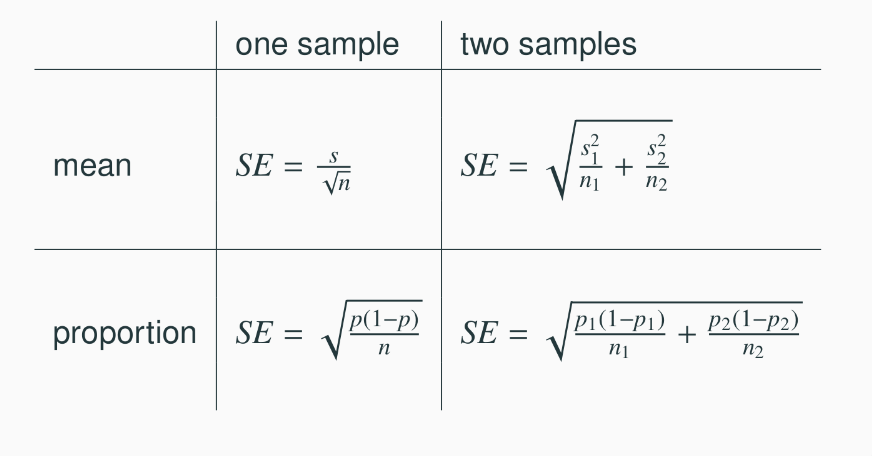
\includegraphics[width=650px]{ref_table}

\begin{itemize}
\tightlist
\item
  When working with means, it's very rare that \(\sigma\) is known, so
  we usually use \(s\).
\end{itemize}

\end{frame}

\begin{frame}{Reference - standard error calculations}
\protect\hypertarget{reference---standard-error-calculations-1}{}

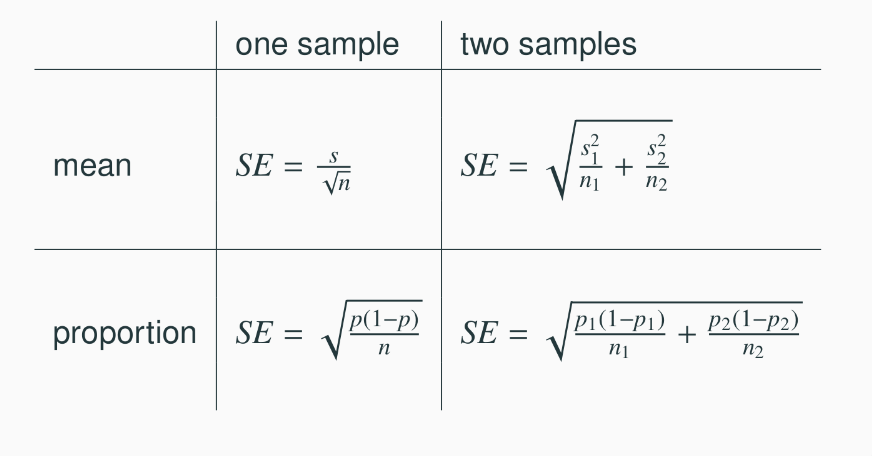
\includegraphics[width=650px]{ref_table}

\begin{itemize}
\tightlist
\item
  When working with means, it's very rare that \(\sigma\) is known, so
  we usually use \(s\).
\item
  When working with proportions,

  \begin{itemize}
  \tightlist
  \item
    if doing a hypothesis test, \(p\) comes from the null hypothesis
  \item
    if constructing a confidence interval, use \(\hat{p}\) instead
  \end{itemize}
\end{itemize}

\end{frame}

\end{document}
